\chapter{Software and Simulation}\label{chapter3}

\newcommand{\SimG}{\texttt{SimG4}\xspace}
\newcommand{\oaEvent}{\texttt{oaEvent}\xspace}
\newcommand{\Geant}{{\sc Geant4}\xspace}

% \begin{markdown}
% ---

% + Introduce ICEDUST, the COMET software suite
%     + Describe whole, then individual parts
%     + oaEvent
 
% + Important part of the software is the set of simulation tools
%     + COMET geometries
%     + Physics, "physics list"?
%     + Show signal event display
%     + SDs, CDC hit representation
%     + RooTracker files
%     + Proton beam input?
%     + Hit merging and bunch simulation
%     + Large-scale production, MC5: Sampling world, example of results?
    
    
% + Version control
% + Continuous integration (+ CD, docker containers)
    
% + Mention miscellanous contributions:
%     + Beginner's tutorial (installation, simulation, analysis)
%     + Move from CMT to CMake and from ROOT5 to ROOT6
%     + Memory leaks and errors
%     + Backward MC: perhaps just ref chapter

% + Animated visualisation of CyDet activity

% ---
% \end{markdown}

Experiments in high energy physics are commonly accompanied by the development of a set of software tools to help in manipulating and analysing experimental data. Simulations are used intensively to optimise experimental designs and prepare for the collection of real data while the physical instruments --- detectors, magnets, readout electronics and data acquisition systems --- are built and assembled.

\section{The ICEDUST Software Suite}
The COMET Collaboration develops a suite of software packages named ICEDUST to satisfy the offline requirements of the experiment. Originally forked in 2013 from the software written for T2K's near detector system ND280, ICEDUST supports the needs of the COMET experiment with regard to simulation, on-disk data format, calibration, reconstruction and analysis.
To fulfil these roles, ICEDUST is divided into specialised packages, as depicted in Fig.~\ref{fig:icedust_schematic}.

\begin{figure}
    \centering
    \hl{TODO}
    %\includegraphics{}
    \caption{The ICEDUST package structure.}
    \label{fig:icedust_schematic}
\end{figure}

\subsubsection{Data format}
At the heart of ICEDUST is the \oaEvent package, which describes the format endorsed by simulation and real experimental data. Based on the ROOT~\cite{BRUN199781} serialisation system, \oaEvent defines a file format where data is laid out as a sequence of events, shown in Fig.~\ref{fig:oaEvent}. The term ``event'' here is purposefully abstract, as the information held in each event can vary. In simulations, an event can describe the outcome of a single proton-on-target (POT) collision, or the outcome of a full proton bunch ($16\times10^6$ POT). 
In data-taking runs, the definition of event will typically be dictated by the data acquisition system.  % So?
\hl{Mention MIDAS for the online data format here.}

\begin{figure}
    \centering
    %\includegraphics{}
    \hl{TODO}
    \caption{Layout of the \oaEvent format.}
    \label{fig:oaEvent}
\end{figure}

Each event is its own hierarchical ``directory'', where data containers can be stored and retrieved by name. The containers themselves are variable-length arrays of arbitrary data types---defined as C++ classes---where objects of the same type can be aggregated.

%The \oaEvent package ties together the processing chains of real and simulated data by providing a unified format understood by all other ICEDUST modules.

% Feels like a big jump. Ease into the real-data processing chain

% Maybe relate back to the figure, take Ben's for placeholder, i.e. in the top left, the simulation chain is composed of X, Y and Z.

When COMET begins collecting experimental data, the raw information will first be stored through the MIDAS format. 
As shown in the \hl{XX loc} of Fig.~\ref{fig:icedust_schematic}, ICEDUST provides utility to convert MIDAS binary data into \oaEvent files. Data in the \oaEvent format can then flow down the chain of calibration, reconstruction and analysis.
The calibration step uses pre-established calibration databases for each sub-detector to convert the digitised information into physical information such as the energy deposit and time that constitute hits. The reconstruction algorithms process hits to find tracks and filter out background, to pass that information down to the final analysis stage.


\section{Monte Carlo Simulation}
Monte Carlo (MC) simulation is the process through which hypothetical particles are realistically propagated through a hypothetical experimental setup, with the aim of evaluating the experiment's performance and to prepare for its realisation. Currently in COMET, MC simulations are heavily used to further optimise the experiment's design and to develop reconstruction and analysis techniques.
%Once real data has been acquired, it can be compared to MC predictions to search for discrepancies indicative of a 

Monte Carlo simulation in high energy physics can be described as the stepwise propagation of particles through matter and electromagnetic fields. Starting from initial conditions of position and momentum, a particle advances in space and time according to the laws of relativistic kinematics. It can change velocity or direction, and produce secondary particles via interactions with the local medium and field. It dies by decaying freely, being absorbed by the material, or exiting the simulation space.
Interactions and decays happen stochastically according to measured tabulated cross-sections and lifetime.

%In a real experiment, detection occurs when energy is deposited inside an active element of the detector. 


In ICEDUST, the \SimG package is responsible for running MC simulations in the different COMET environments. This module handles the parsing of geometry macros and field maps, through which the experimental setup and electromagnetic field are defined. It depends on the \Geant~\cite{AGOSTINELLI2003250} particle simulation toolkit to propagate particles and throw the dice on interactions and decays.

\section{Geometry}
\Geant allows the definition of complex volumes from simple polygons via its set of constructive solid geometry classes.
The \SimG package extends \Geant's macro language to allow geometrical parameters to be defined in macro files. The position, dimensions, and material of every volume can thus be specified at run-time rather than compile-time. The custom macro parser allows parameters to depend upon other parameters, and supports looping, for instance to position identical elements in a regular pattern.

%Once the whole geometry is assembled, it is translated into an equivalent ROOT representation that will be stored into the output file for book-keeping. This copy can also be rendered more readily by the 3D utility classes of the ROOT package. % Link to DisplayCore? !! REMOVED --> out of scope of section?


All three COMET setups, Phase-$\alpha$, Phase-I and Phase-II, have been implemented in fine detail in the \SimG package, allowing faithful simulations to be performed to predict the COMET experiment's performance. % too much?
Fig.~\ref{fig:comet_geometries} shows renderings of the two COMET setups to be used in the search for CLFV.

\begin{figure}
    \centering
    \captionsetup[subfigure]{justification=centering}
    % To make this figure: thin wireframes, white background
    % Plane clipping at y=10
    % zoom all the way out and move the camera forward (right-click)
    % so the perspective approaches an isometric view.
    \begin{subfigure}[t]{0.49\textwidth}
        \centering
        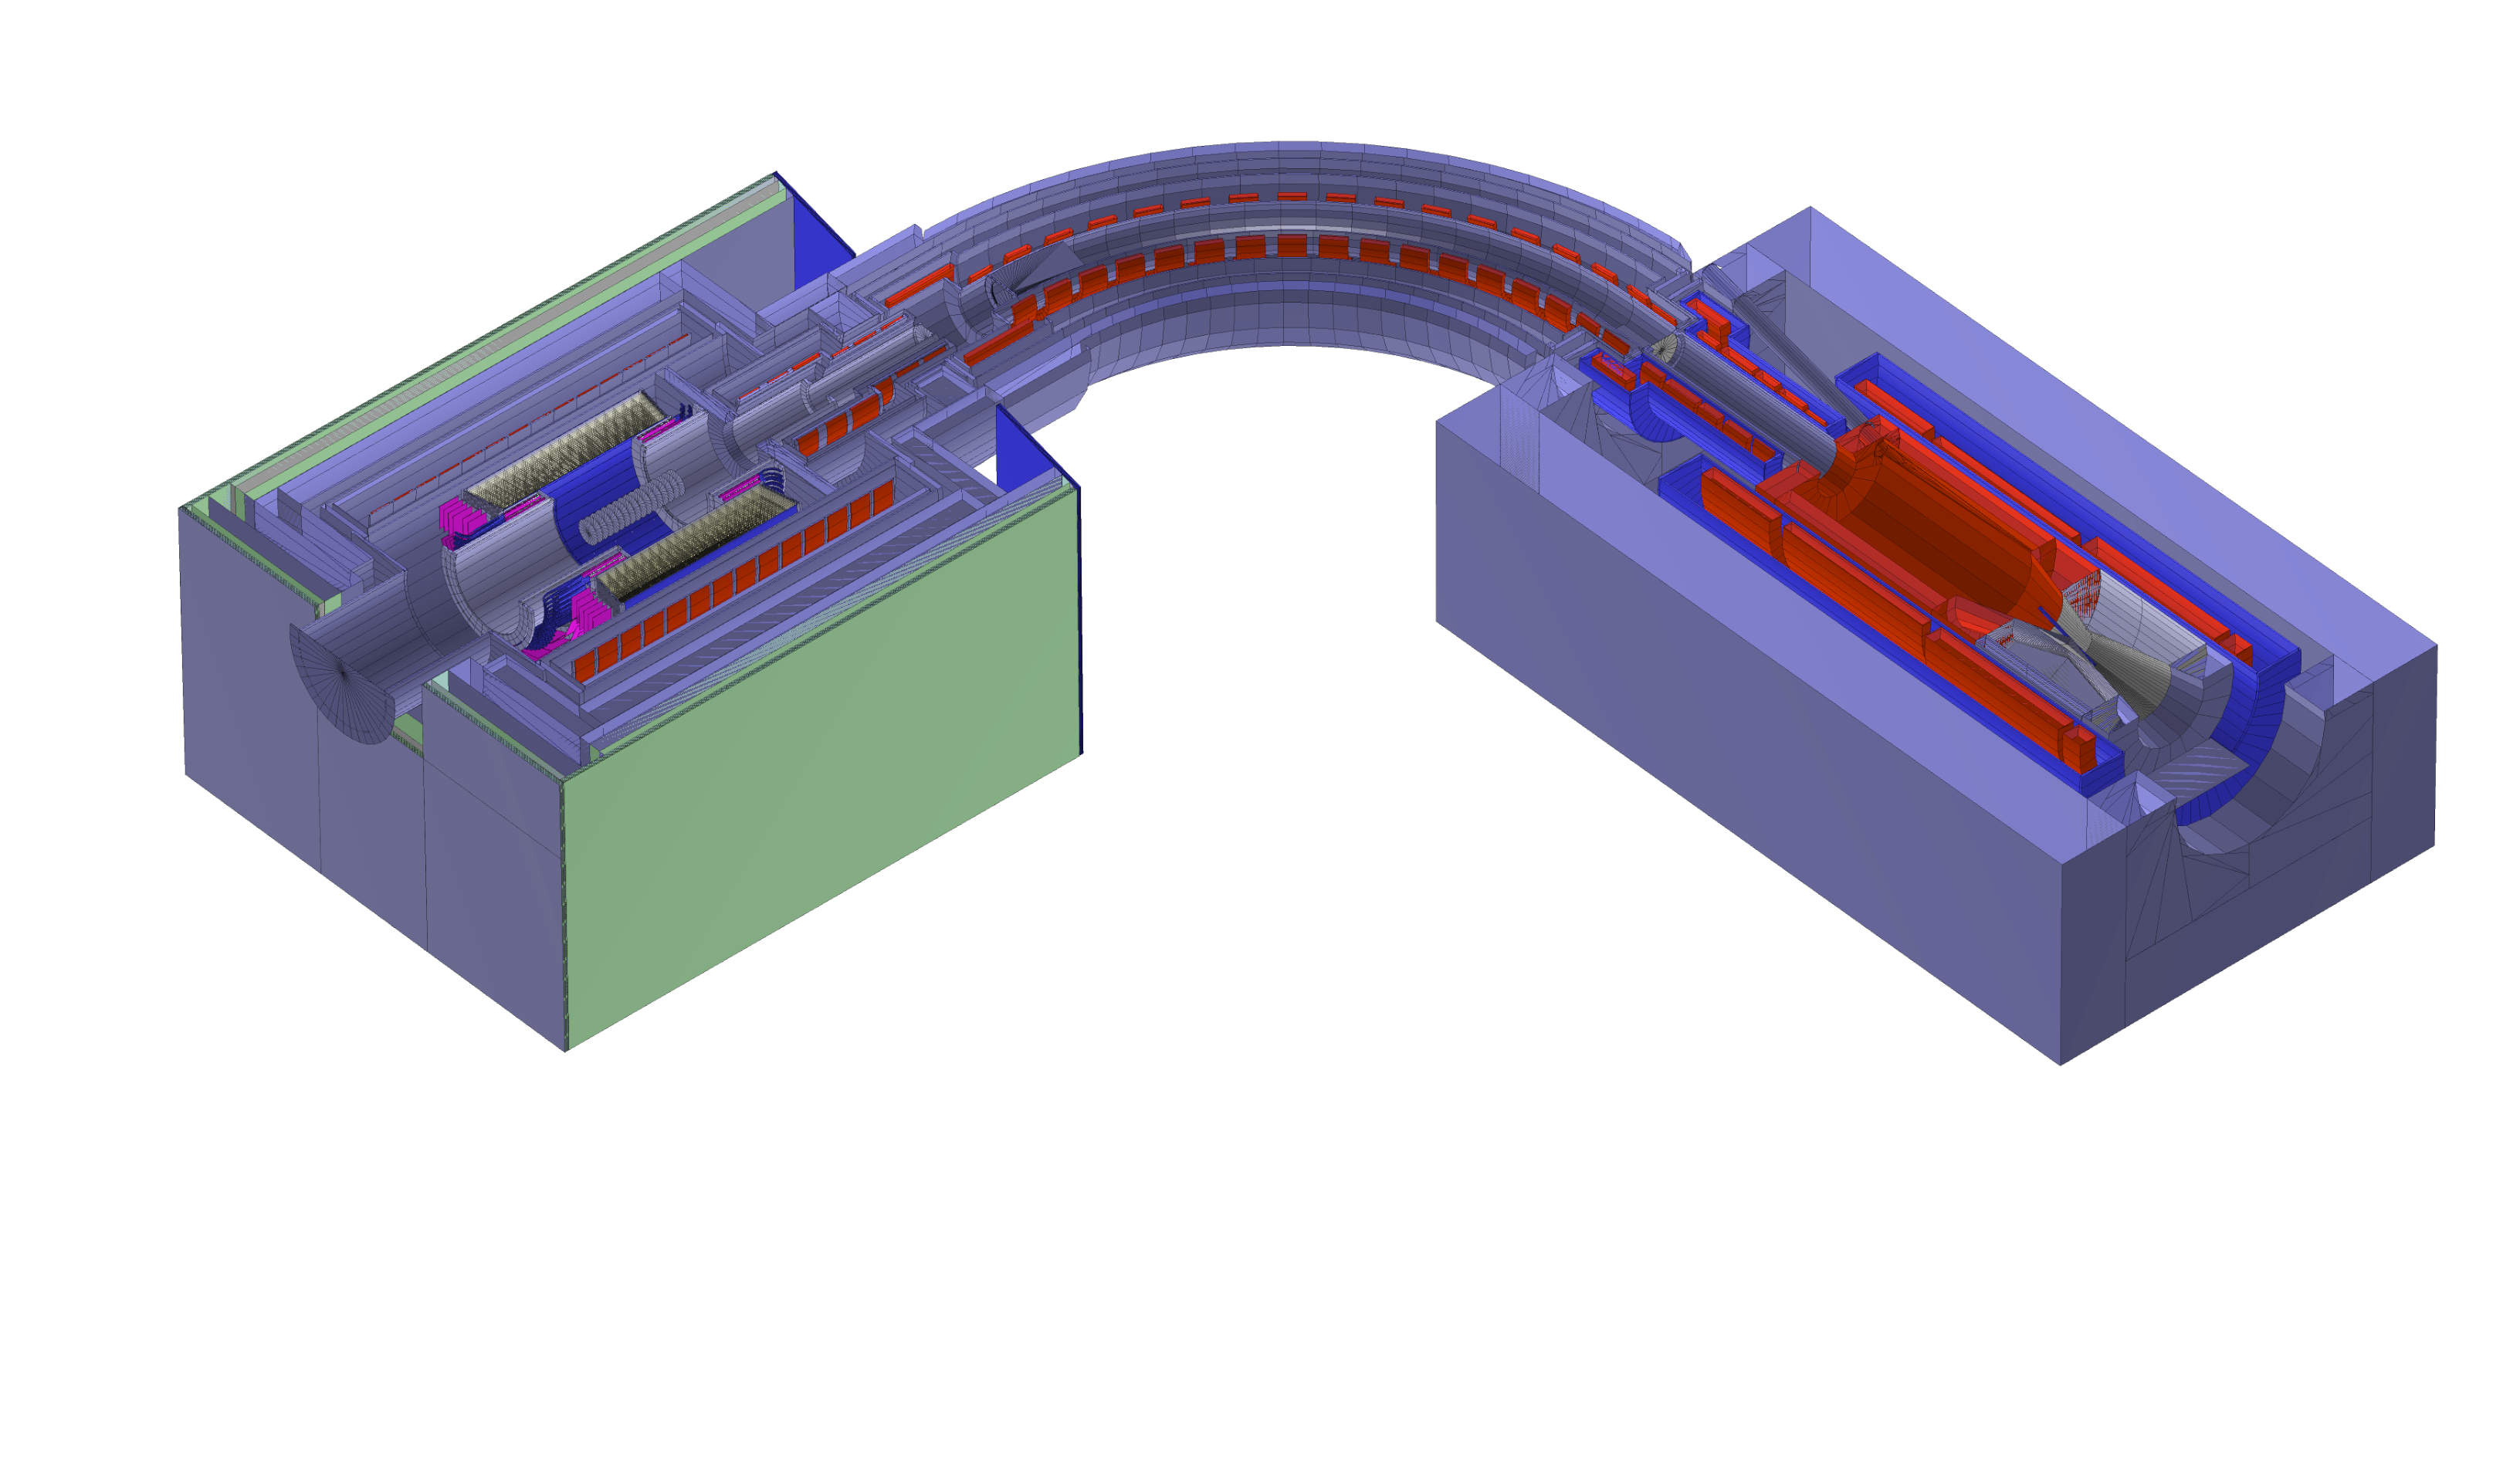
\includegraphics[width=0.95\textwidth]{chapter3/geometries_Phase-I_iso_cropless_huesat.png}
        \caption{Phase-I in the CyDet configuration.}
    \end{subfigure}
    \hfill
    \begin{subfigure}[t]{0.49\textwidth}
        \centering
        \includegraphics[width=0.95\textwidth]{chapter3/geometries_Phase-II_iso_huesat_nohuman.png}
        \caption{Phase-II.}
    \end{subfigure}
    
    \caption{Cutaway views of the simulation geometries implemented in \SimG and visualised with \texttt{DisplayCore}. The experiment hall is also modelled in the simulation but was hidden here for clarity.}
    \label{fig:comet_geometries}
\end{figure}

% Event generation 
\section{Event generation and bunch structure}
Protons are sampled from a beam profile histogram at a distance of \SI{70}{\cm} upstream of the target. The histogram is generated via a Turtle~\cite{Carey1974DecayT} simulation of the proton beamline.

In the simulation, a single proton is sampled from the beam histogram for each event, which differs from the real situation in that the actual beam is arranged into bunches, each containing about 16 million protons. Hence we assume that proton collisions in a bunch are independent of each other, and we merge POT events into bunch events by overlaying the produced trajectories and hits. This task is handled by the \texttt{SimHitMerger} program. The structure of the proton bunch can be parametrised by various functions, the most common of which is a square-wave shaped timing structure with a width of \SI{100}{\ns}. For each POT event, all trajectories and hits are shifted by a uniformly sampled timing offset between -50 and \SI{50}{\ns} to simulate the bunch structure. 

\section{Physics}
The COMET experiment involves many physical processes to go from the initial proton collision to backgrounds in the detector.
The MC simulation must faithfully account for any process which could lead to backgrounds if we are to realistically estimate the experiment's sensitivity. The \SimG simulation associates standard \Geant hadronic and electromagnetic physics lists with custom logic for nuclear muon capture and muon decay-in-orbit.

To model hadronic interactions, \SimG uses the \texttt{QGSP\_BERT\_HP} reference physics list. Hadron-nucleus interactions between the \SI{8}{\GeV} proton beam and the pion-production target are handled by the Bertini Cascade model~\cite{WRIGHT2015175}.

Muons at rest receive special treatment in the COMET simulation due to their important contribution toward the background rate. The default energy spectrum of electrons from muon decay-in-orbit is replaced by the numerical evaluation of~\cite{czarnecki}, which includes the effect of nuclear recoil and thus allows electron energies up to \SI{104.973}{\MeV}. In addition, the nuclear muon capture (NMC) model is replaced to adhere to the results of the AlCap experiment~\cite{litchfield2015status}, where the frequency of proton emissions after NMC in an aluminium target was measured as well as their energy spectrum.


\section{\hl{POSITION}}

\subsubsection{Virtual monitors / oaRooTracker}
% RooTracker files
The simulation software provides utility to record particles that reach certain key points in the geometry, such as the transport solenoid or the detector region. Virtual monitors are volumes that can be placed in the geometry to record the passage of particles, in the form of virtual hits or into a separate file. The file format used to save particle states is called \texttt{RooTracker}. It stores the kinematics of simulated particles and can thus be used as input to another simulation run. % and?




\section{Signal simulation}
By default, the list of physical processes considered by \SimG includes only SM-allowed interactions and decays, and hence does not include $\mu$--$e$ conversion. In order to simulate signal events, one can manually produce conversion electrons out of the muons stopped inside the stopping target.

From the normal beam simulation, one can estimate the spatial distribution of muons stopped in the stopping target and subsequently sample conversion electrons from it. In sensitivity studies, signal events are commonly overlaid onto a pure background sample in order to evaluate the signal acceptance and background rejection efficiencies of the hit filtering and track finding routines. % Accurate?

\begin{figure}
    \centering
    \captionsetup[subfigure]{justification=centering}
    \begin{subfigure}[t]{0.43\textwidth}
    \centering
    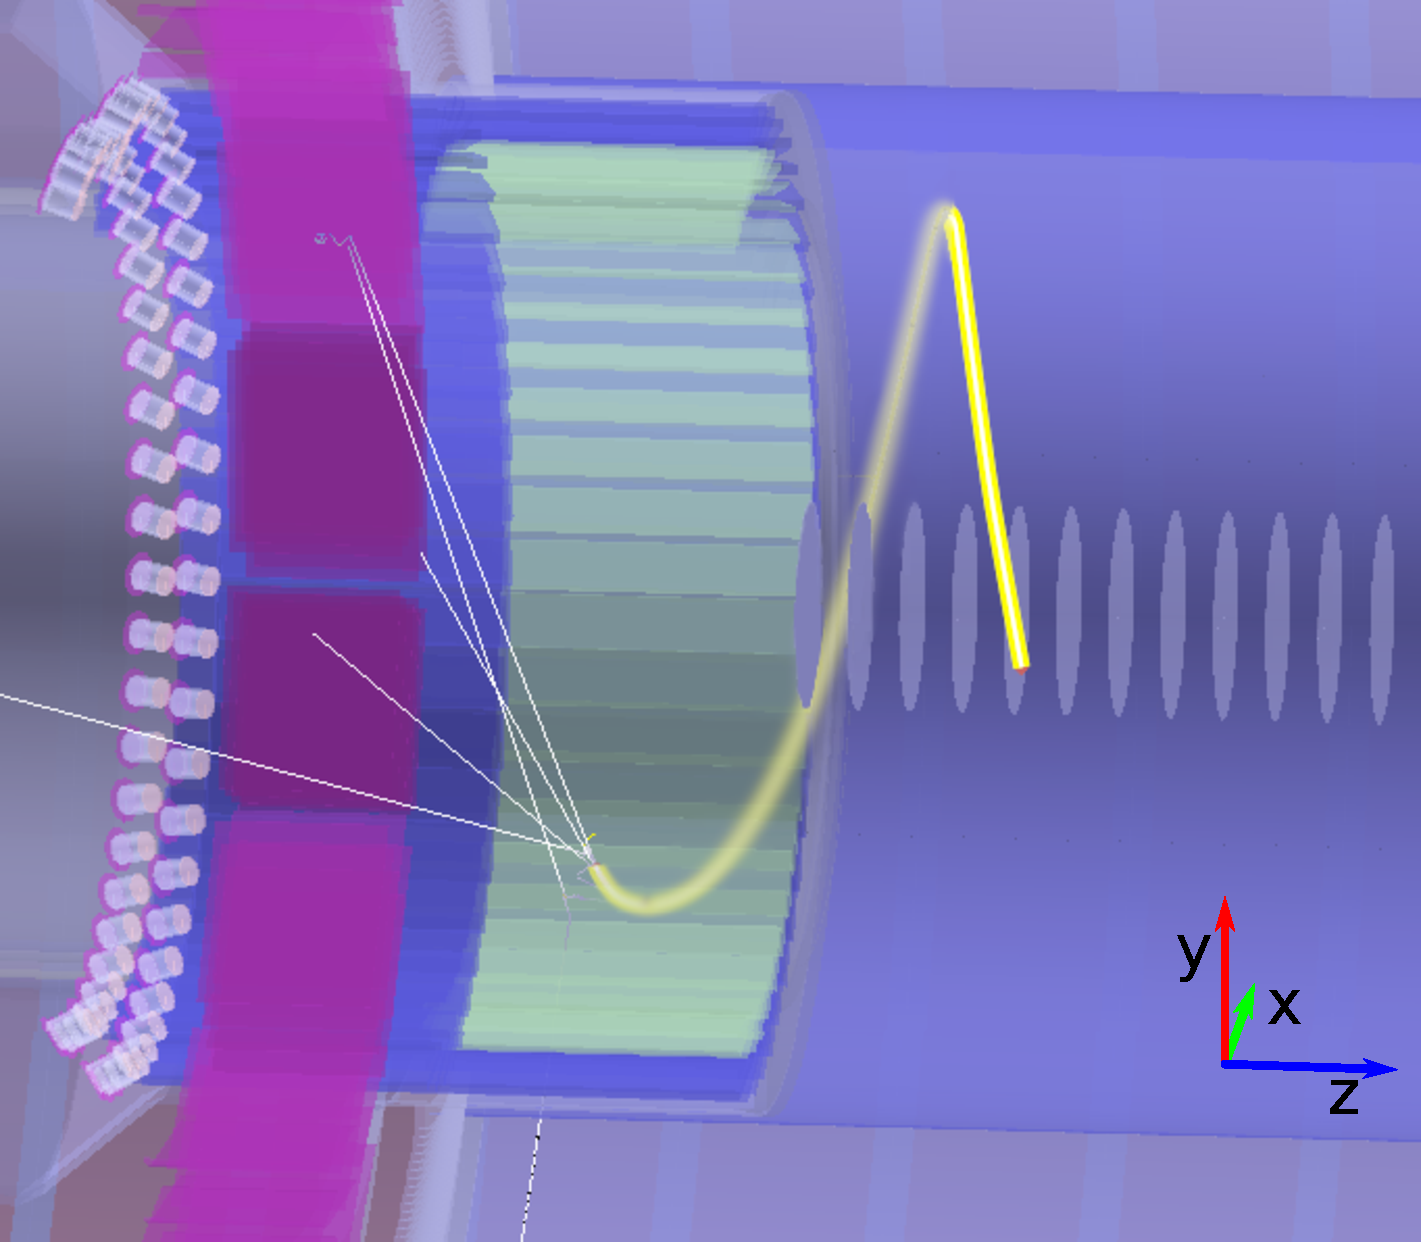
\includegraphics[width=0.95\textwidth]{chapter3/signal_event_display_crop_axes.pdf}
    \caption{Event shown in \texttt{DisplayCore}, the 3D event display.}
    \end{subfigure}
    \hfill
    \begin{subfigure}[t]{0.48\textwidth}
    \centering
    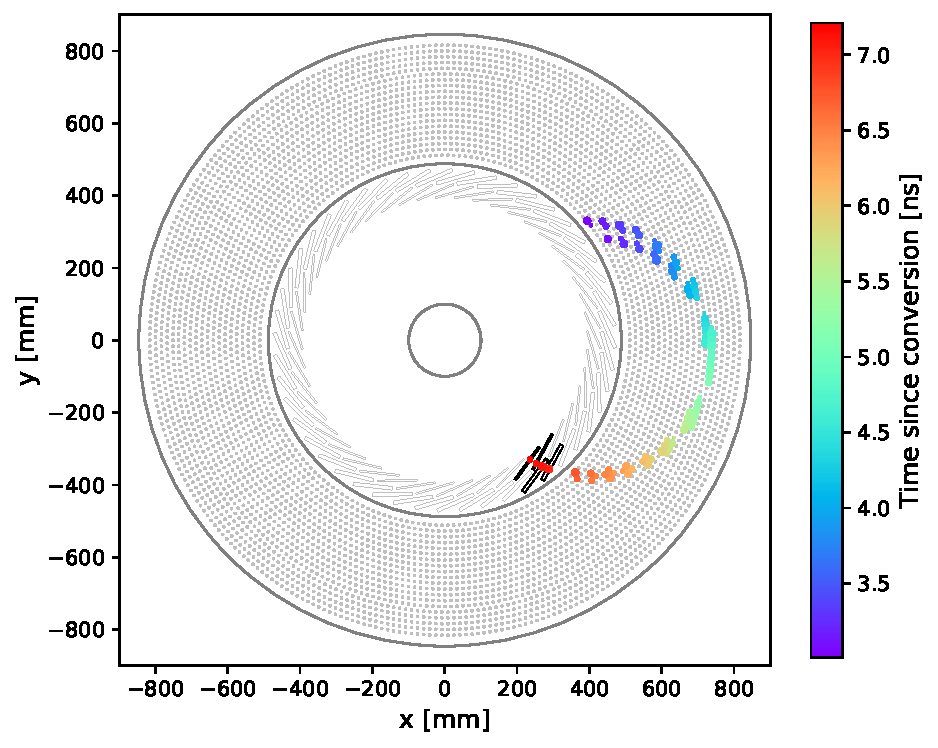
\includegraphics[width=0.95\textwidth]{chapter3/cydet_signal_track_v2.pdf}
    \caption{Event as seen by the CDC and CTH detectors.}
    \end{subfigure}
    
    \caption{Example of a simulated signal trajectory in the CyDet system. This particular event triggers the CTH and would be considered as an ideal candidate of a $\mu$--$e$ conversion signal.}
    \label{fig:signal_event}
\end{figure}

Fig.~\ref{fig:signal_event} shows a simulated conversion electron emerging from the stopping target, depositing energy inside the CDC gas, to eventually trigger the CTH by hitting four adjacent counters. 
The Cylindrical Detector is purposefully designed to maximise the acceptance of such tracks, while minimising that of backgrounds \hl{(discussed in chap~2)}.% Necessary?

\section{Detectors and hits}\label{subsec:SD}
% Sensitive detectors, truth-hit representation
In \Geant simulations, particles are individually tracked---propagated step by step in space and time---through materials and electromagnetic fields. 
As a particle interacts with elements of the geometry, it tends to lose energy to the medium, e.g. through inelastic scattering or ionisation. 
Usually, these energy deposits are of little importance, however they must be recorded inside active detector elements in order for us to determine the response of the detector and readout systems to the passage of the particle.
%By knowing the position, time and energy lost by particles, the response of the detector can be simulated.

% Detector response example? E.g. in the CDC, knowing charge, position and time allows us to calculate the amount of charge collected onto each wire, and thus with knowledge of the readout electronics architecture, we can convert this to a digitised readout.

Detector elements in \Geant are defined as ``sensitive volumes'', and energy deposits of incoming particles are accumulated and recorded as ``hits''. 
The way in which we represent hits is typically dependent on the type of detector, meaning for instance that we treat the response of a plastic scintillator in a different manner from that of a gas chamber. % Confusing?

In early 2019, ICEDUST developers agreed to change the definition of hits inside the CDC gas volume in order to more accurately portray the energy deposit information in that detector. Along that process, I came to be thoroughly involved in the testing and refinement of this new CDC hit representation, named \texttt{IG4HitGas}. 

A hit representation is formulated as a C++ class which holds the hit's data. It must be coupled to a sensitive detector class, whose role is to receive information from \Geant's particle tracking system and accumulate it into instances of the hit class. For example, the sensitive detector class for a calorimeter might produce hits containing the total energy deposited for each inbound particle as well as a timestamp.

\begin{figure}
    \centering
    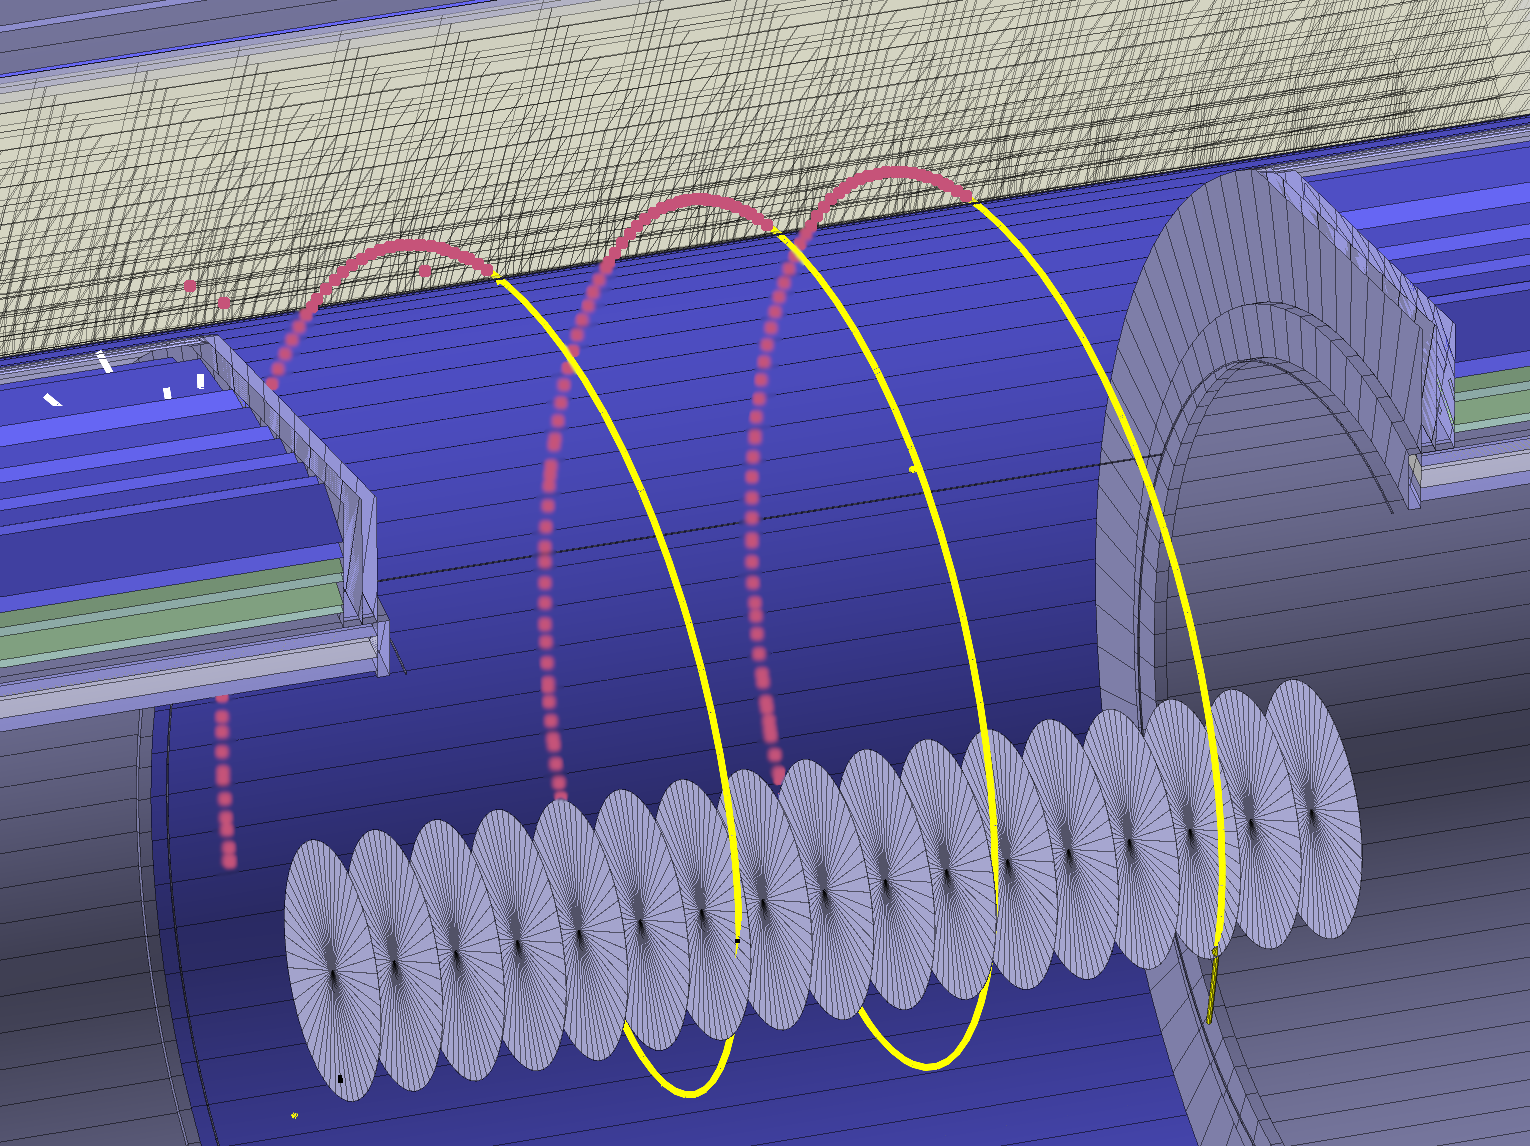
\includegraphics[width=0.5\textwidth]{chapter3/hit_instances_blur_crop.png}
    \caption{Hits, shown as red dots, produced by the CDC's sensitive detector class when a particle deposits charge inside the gas. One instance of \texttt{IG4HitGas} is created every time the particle traverses a CDC cell.}
    \label{fig:sim_cdc_hits}
\end{figure}

The \texttt{IG4HitGas} class was designed to condense and record energy loss information inside gaseous ionisation detectors in \SimG (e.g. the CDC and Straw-Tube Tracker). Every energy deposit made by a particle inside the same CDC cell is accumulated into a single instance of the class, such that only one hit per cell per particle may exist. While this saves memory and disk space, it limits the amount of detail that can be stored. The recorded information allows for basic detector response simulation, but if more detail is required one can tune the \SimG simulation to store finer details inside each \texttt{IG4HitGas} instance.

Fig.~\ref{fig:sim_cdc_hits} shows the position of \texttt{IG4HitGas} instances along an electron's trajectory in the CDC.


\section{Large-scale simulation: MC5}\label{sec:mc5}
In early 2020, I was responsible for running a large-scale production of MC simulation data, called MC5, using computing facilities at the French National Institute of Nuclear and Particle Physics Computing Centre (CC-IN2P3) in Lyon, France.
Using \num{2000} concurrent machines over the course of a few weeks, the outcomes of 1 billion proton-on-target (POT) collisions were simulated with \SimG in the CyDet configuration of COMET Phase-I.

Leading up to this production, many changes took place in the software. The CMake build configuration tool was introduced to replace the now less-standard CMT system. We carried out the switch between major versions of the ROOT package upon which many of our packages depend, most importantly the \oaEvent data format. The CyDet geometry received multiple updates to make it as faithful as possible to the design, adding detailed elements such as readout boards and fixing errors in the positioning of CDC wires. As discussed in~\ref{subsec:SD}, the treatment of energy deposits in the CDC was also changed to better reflect the detector's operation.  % operation right word?
Finally, all memory-related problems identified by \texttt{valgrind} at the time were resolved to bring the simulation software into a production-ready state.

The simulation was split into two stages by dividing the simulation world along a boundary which effectively separates the pion-production section and transport solenoid (upstream) from the detector region (downstream), as shown in Fig.~\ref{fig:Phase-I Sampling World}. In the upstream run, the tracking of particles entering the detector region is stopped and their kinematics are saved to a RooTracker--\hl{reference a section}-- file to be later used for the downstream run. 

This way to proceed means that the upstream simulation is unaffected by the disposition of the detector region, hence one can perform the upstream run once and use the results in multiple downstream configurations, changing the detector geometry (e.g.\ between CyDet and the StrawECAL) or magnetic field. 
Another benefit is that it allows for re-seeding of the downstream run, whereby each event retains the same initial conditions but uses several different seedings of the random number generator, yielding a more diverse dataset at the cost of potentially biasing the sample.
% Perhaps unclear, might need to split the sentences

\begin{figure}
    \centering
    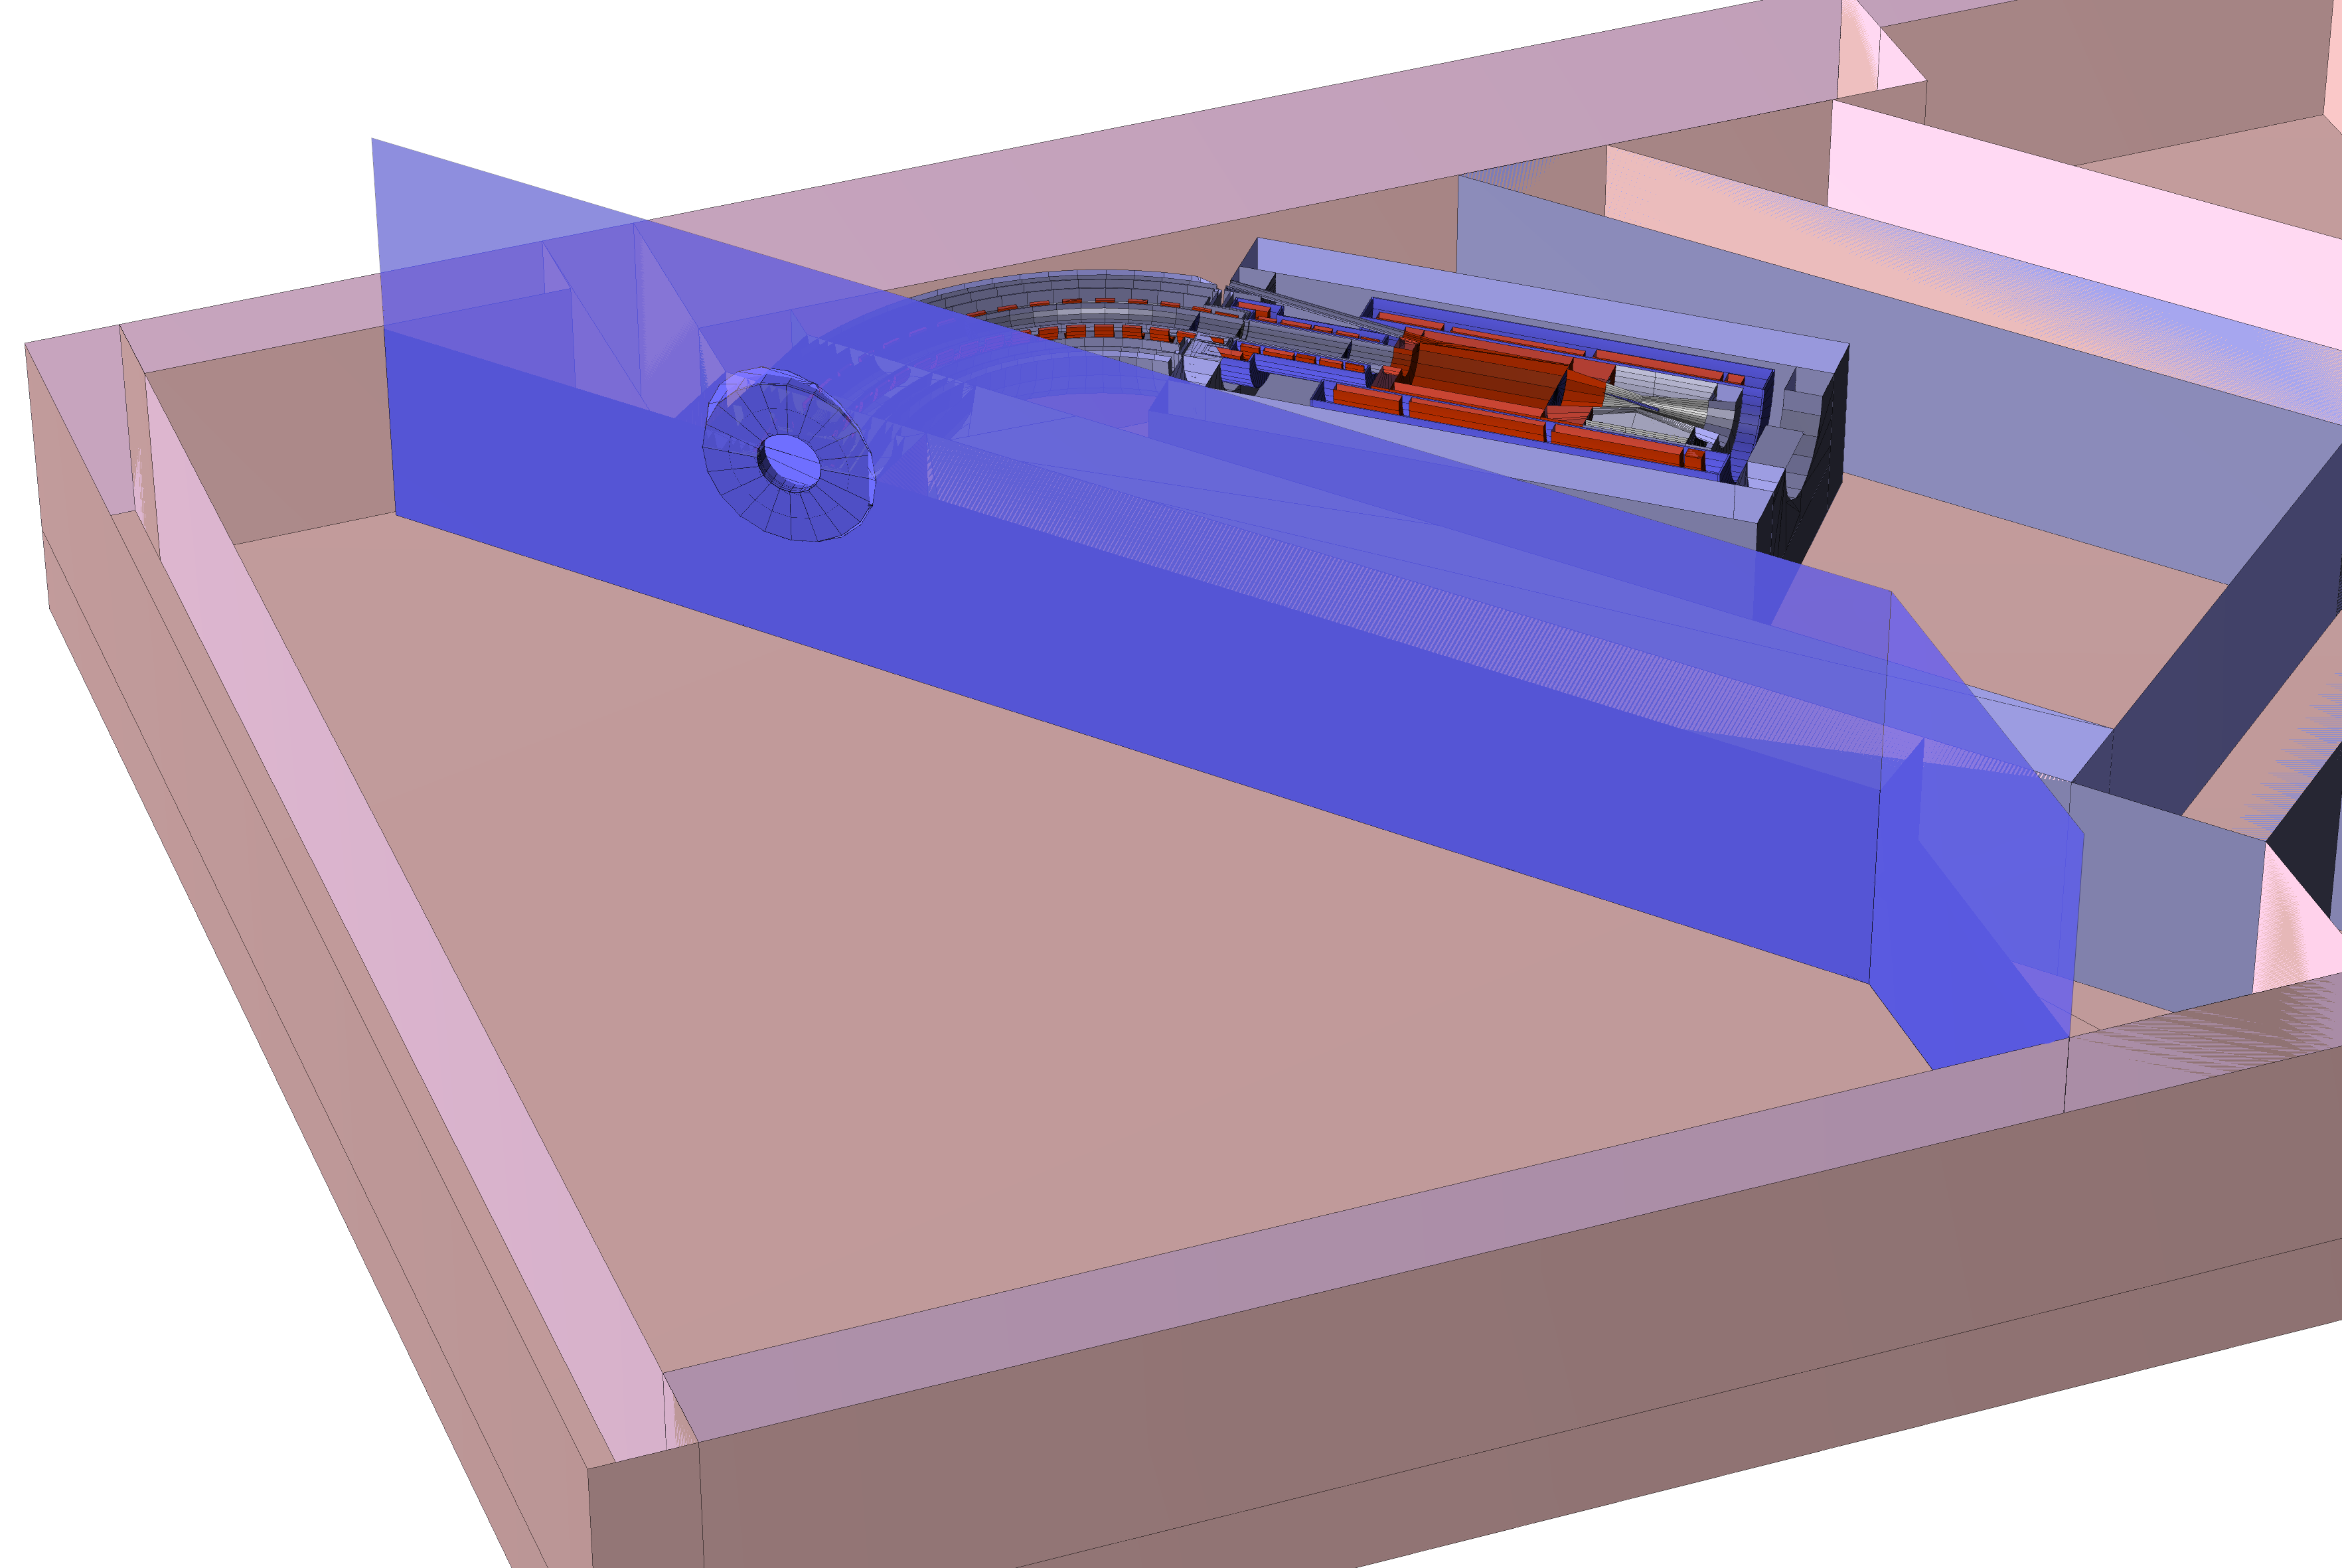
\includegraphics[width=0.6\textwidth]{chapter3/sampling_world_crop_smooth_transparency.png}
    \caption{Rendering of the Phase-I "Sampling" world, where the detector region is empty and only the upstream part of the simulation is performed. The blue surface, along with the floor and ceiling of the detector region, are the boundaries at which particles recorded for the subsequent downstream simulation.}
    % Alternatively: show upstream trajectories and downstream continuation...
    \label{fig:Phase-I Sampling World}
\end{figure}

The data produced for MC5 has a total disk size of \SI{13}{TB} and is archived on the tape storage system at CC-IN2P3.

\section{Animated CyDet event display}
In order to visualise events in the CyDet system, I created a tool to convert hit data from MC simulations into animations resembling an online event display of the detector. Fig.~\ref{fig:animation} shows a series of frames from one such animation involving a $\mu$--$e$ conversion electron.

In the CDC, the true position of every hit is drawn as a circle with a radius proportional to the energy deposited. Colour indicates hits produced by the same particle. Each animation shows one bunch event unfolding over one cycle, i.e.\ \SI{1170}{\ns} from the collision of one bunch until the arrival of the next one, at a greatly reduced speed.
The left-hand side of the animation shows the projection in the readout plane, with the CDC on the outside and the CTH counters on the inside. The right-hand side shows the perpendicular projection so that depth is apparent as well.

The CTH counters do not flash for every energy deposit but only in the case of a fourfold coincidence event. Only if four adjacent counters are struck within a \SI{10}{\ns} window is the coincidence registered and the hits shown. Fourfold coincidences are most often caused accidentally by several particles, but occasionally a single track will hit four counters. In these occurrences, the track is emphasised in the animation and the particle type is displayed.

\begin{figure}
    \centering
    
    \captionsetup[subfigure]{justification=centering}
    \begin{subfigure}[t]{0.49\textwidth}
    \centering
    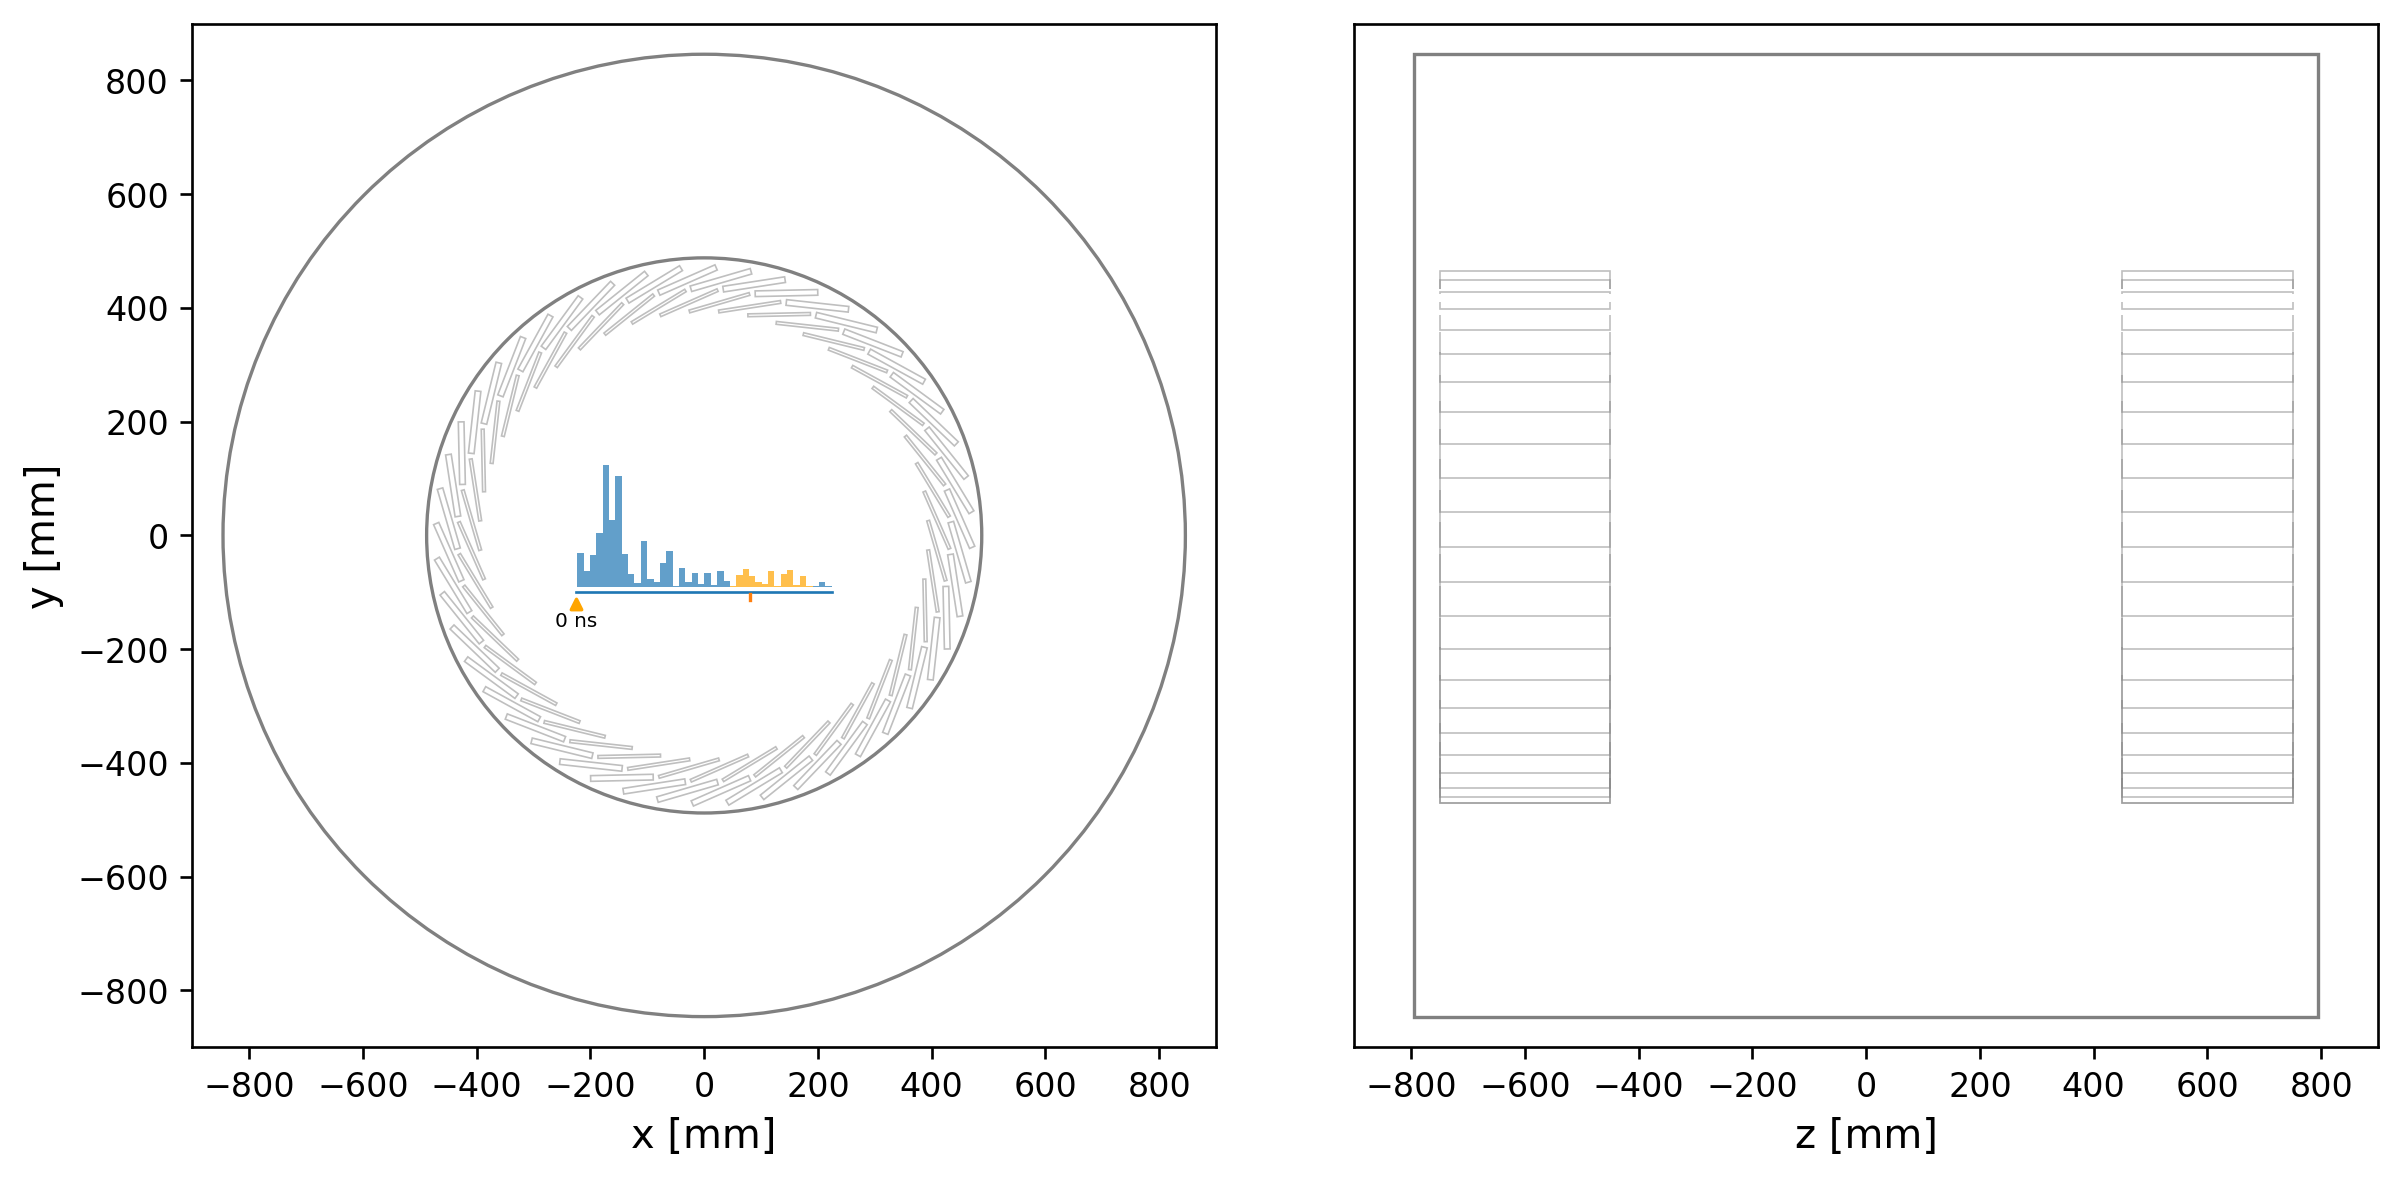
\includegraphics[width=0.95\textwidth]{chapter3/frame_005.png}
    \caption{$t=\SI{0}{ns}$.}
    \end{subfigure}
    \hfill
    \begin{subfigure}[t]{0.49\textwidth}
    \centering
    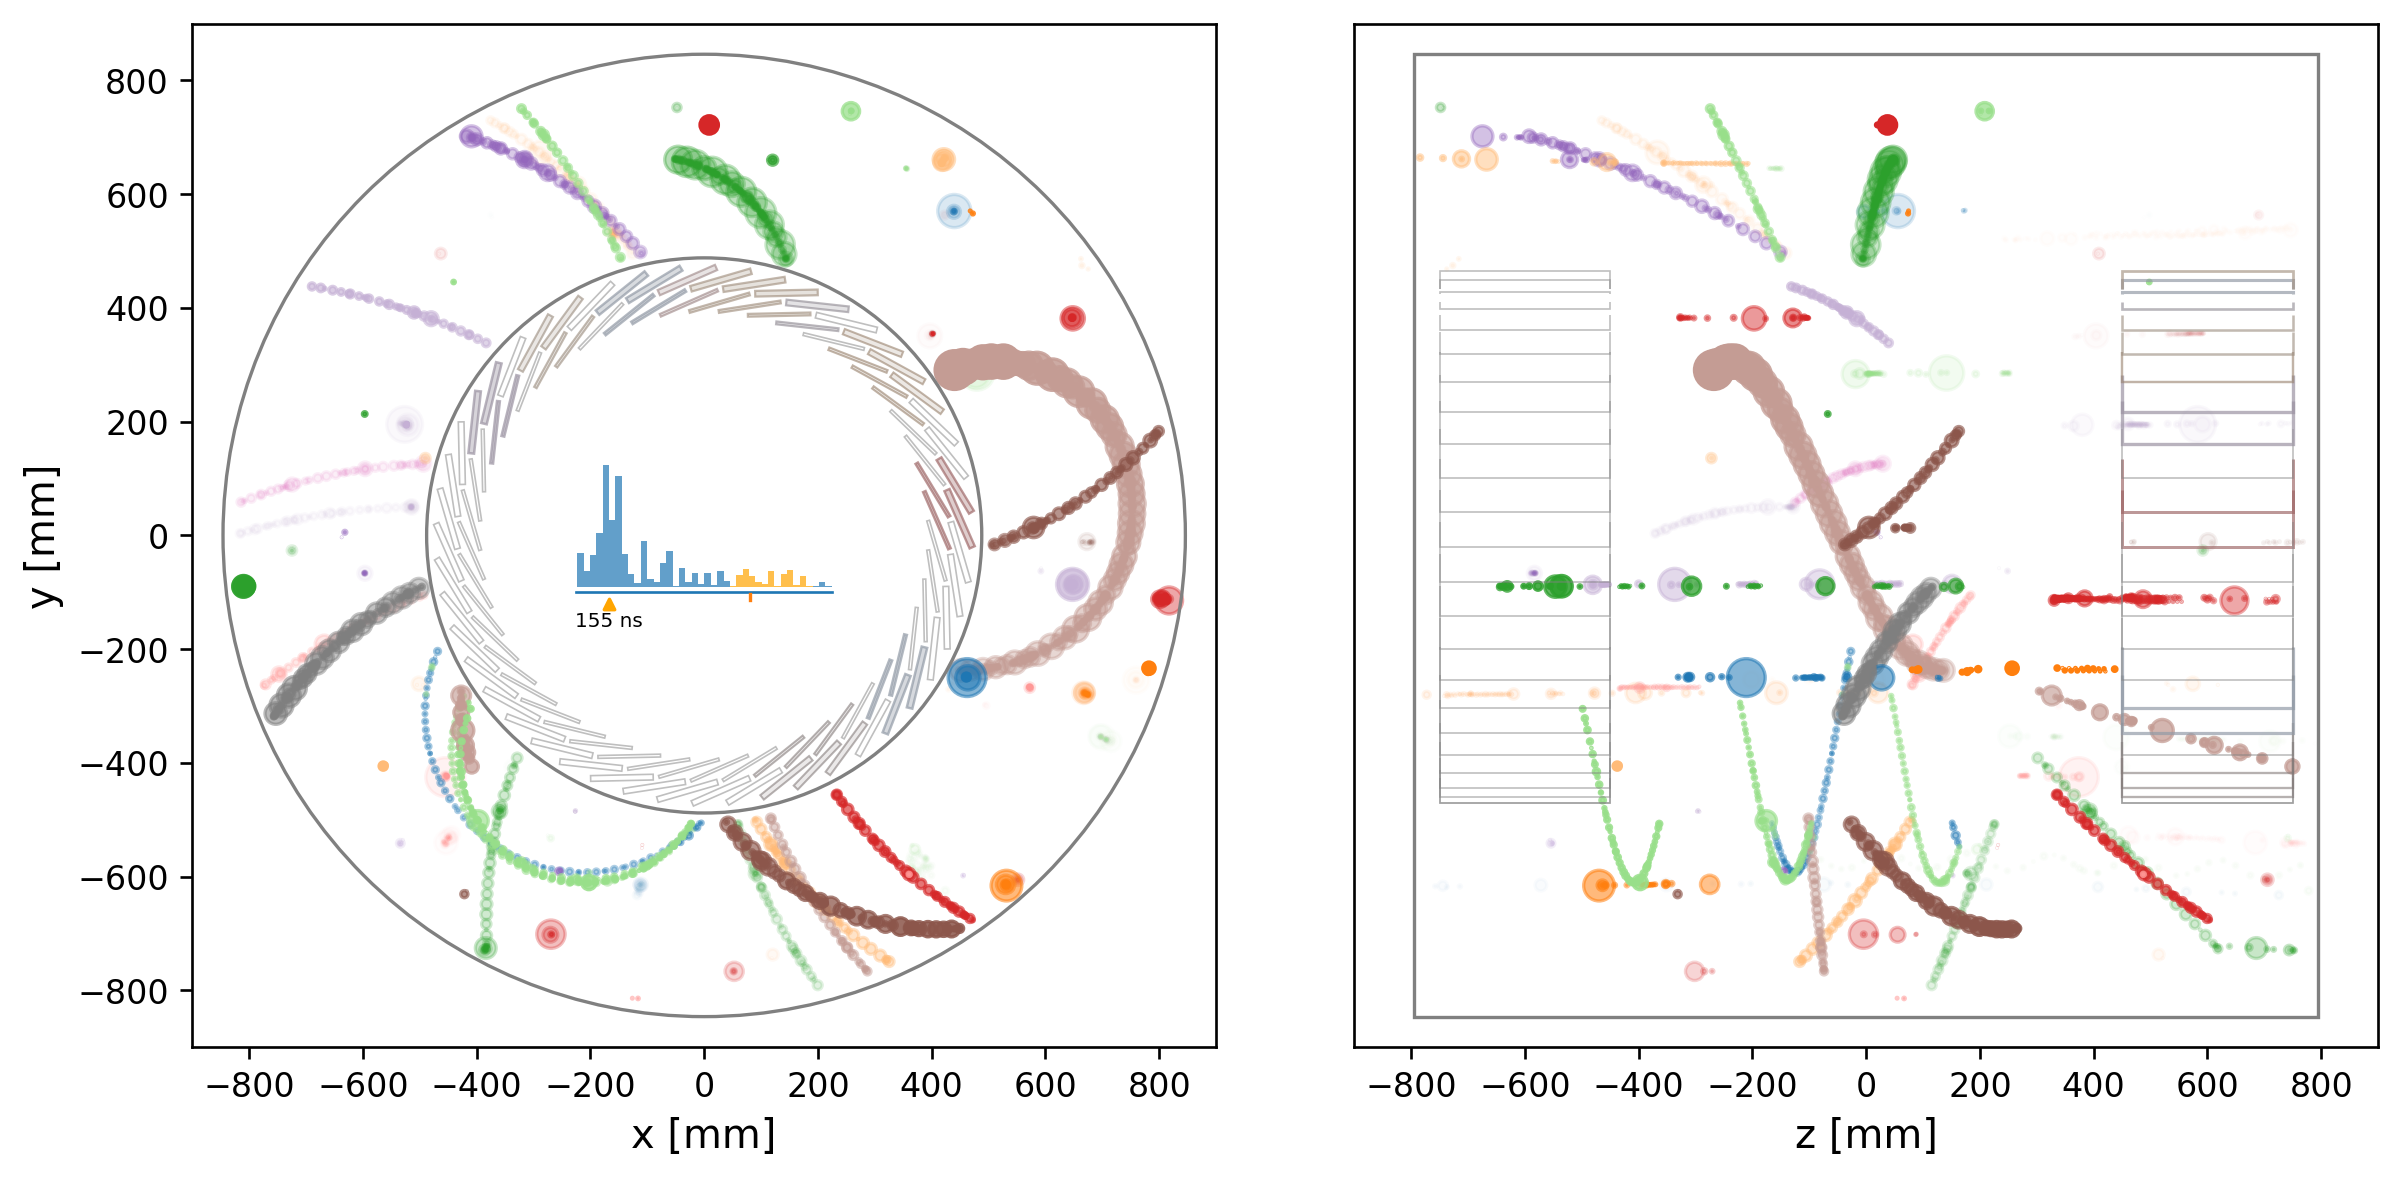
\includegraphics[width=0.95\textwidth]{chapter3/frame_036.png}  
    \caption{$t=\SI{155}{ns}$: many tracks occupy the detector after the beam flash.}
    \end{subfigure}
    
    \vspace{0.3cm}
    
    \begin{subfigure}[t]{0.49\textwidth}
    \centering
    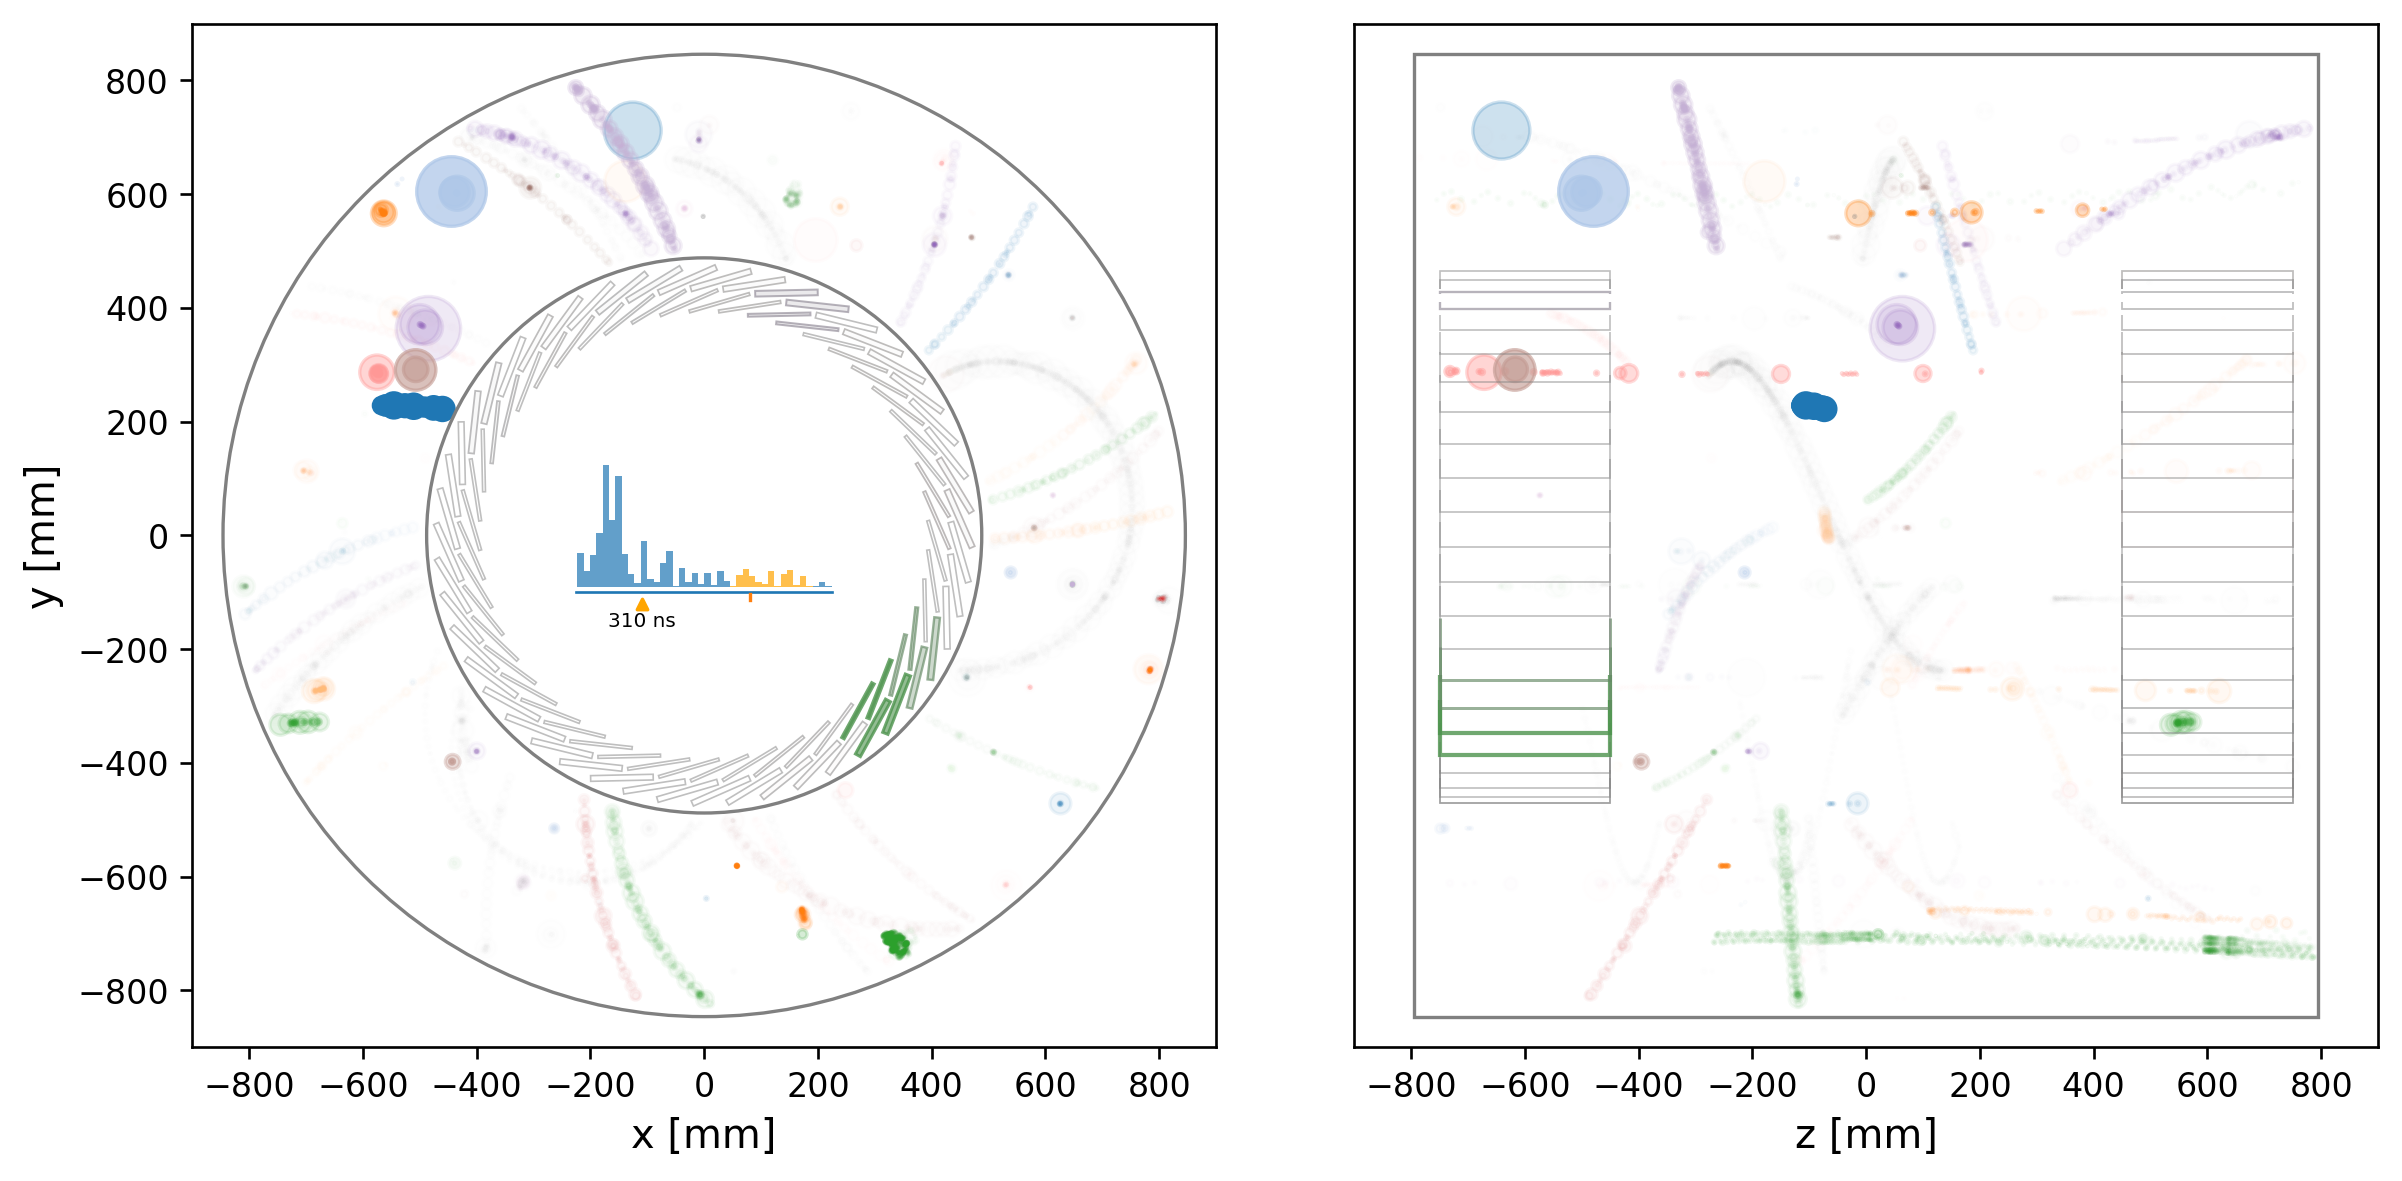
\includegraphics[width=\textwidth]{chapter3/frame_067.png}
    \caption{$t=\SI{310}{ns}$: the hit rate decreases significantly once the beam flash has ended.}
    \end{subfigure}
    \hfill
    \begin{subfigure}[t]{0.49\textwidth}
    \centering
    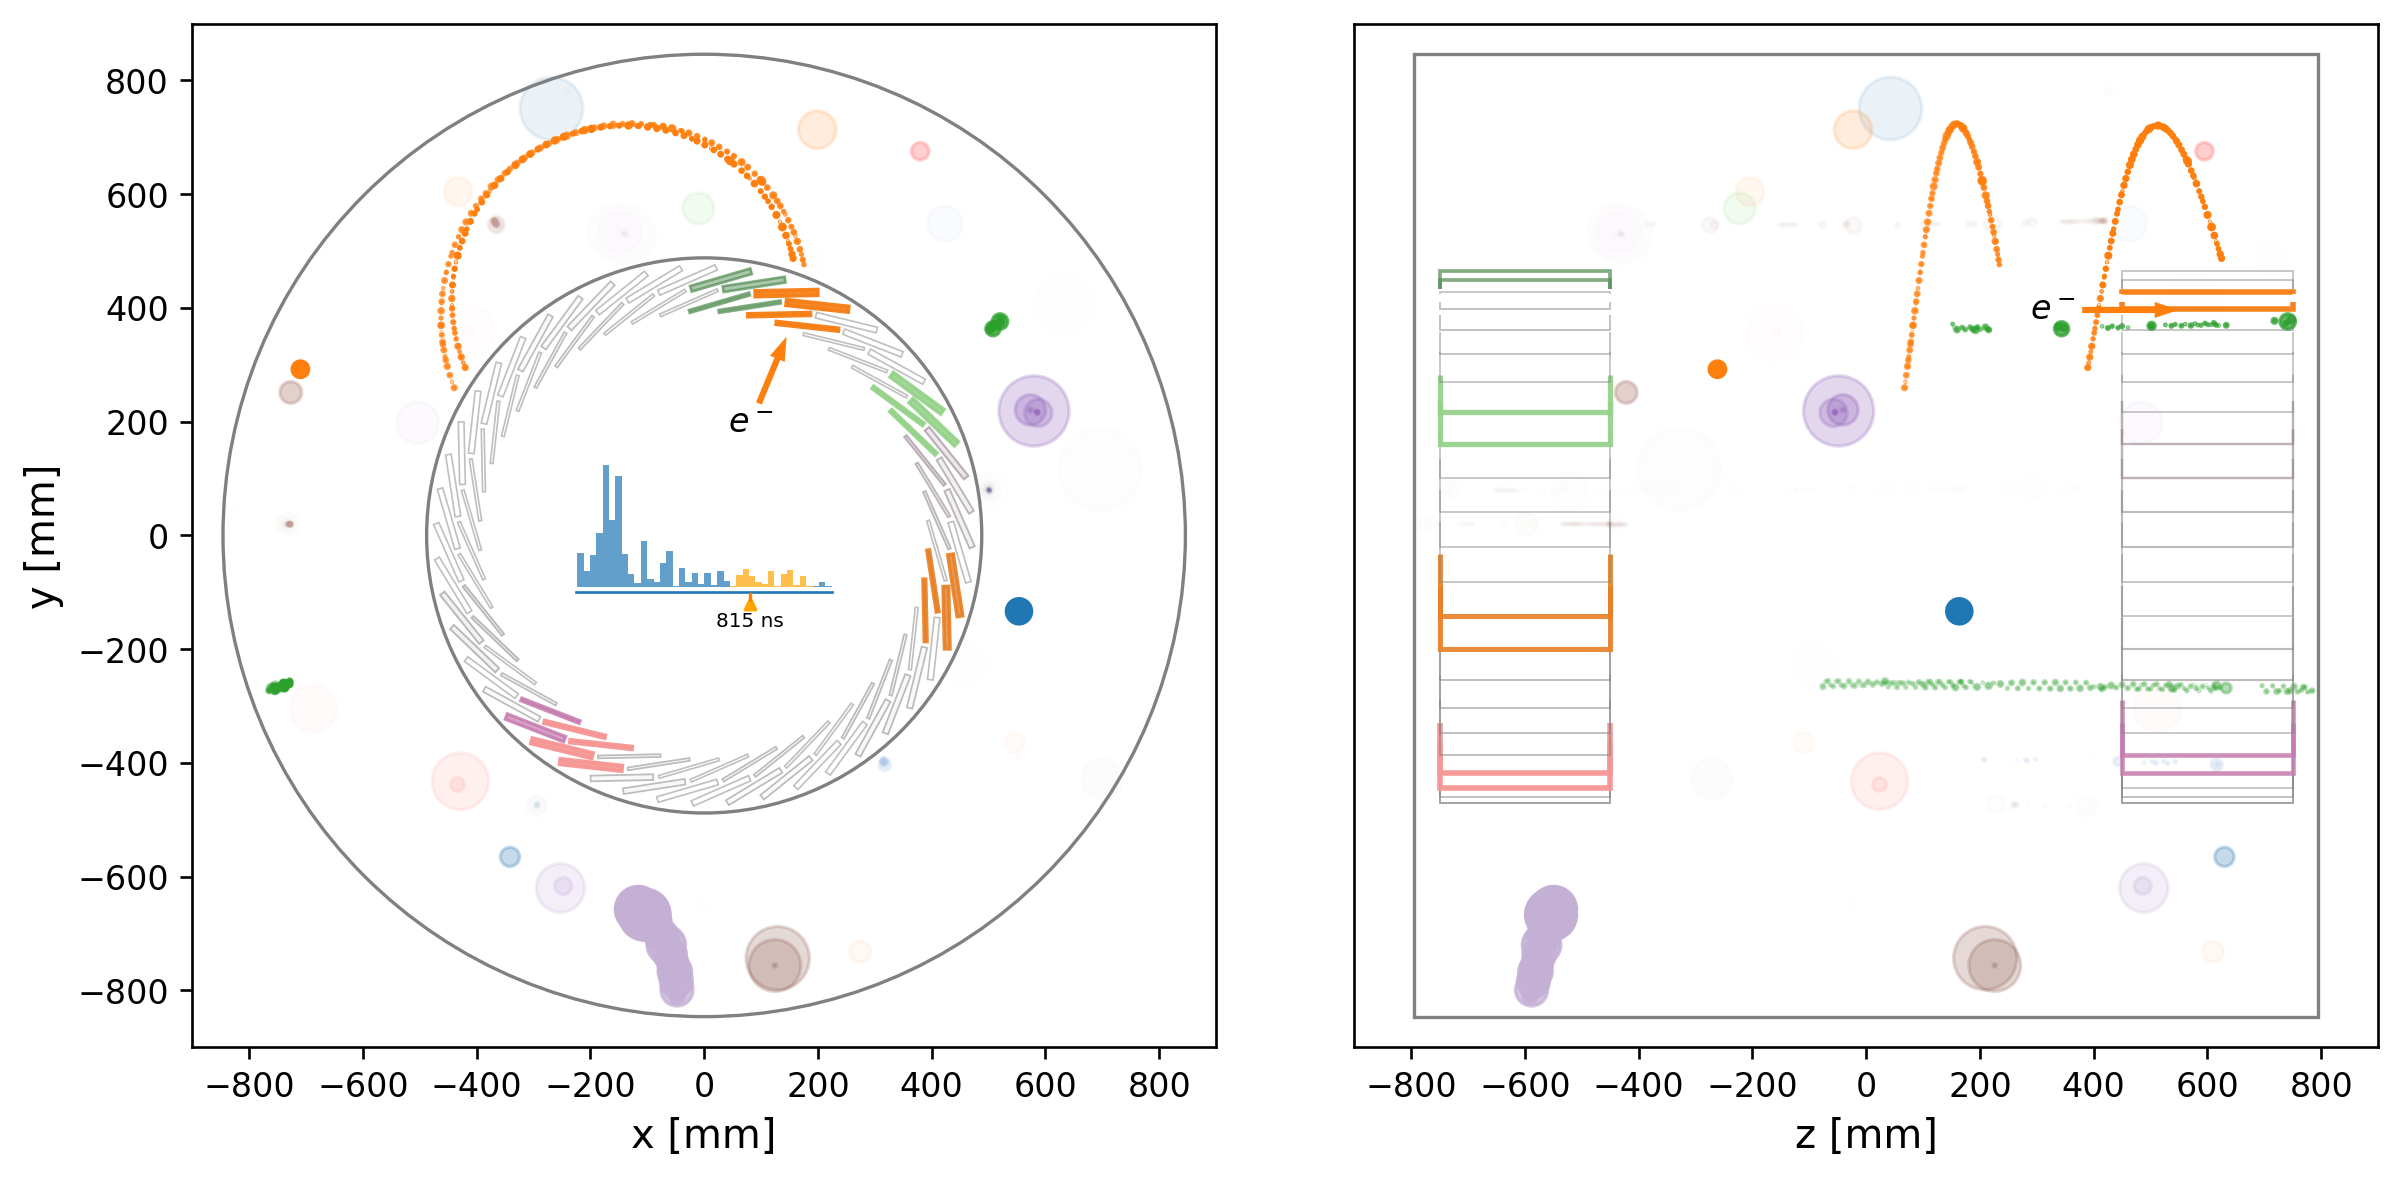
\includegraphics[width=\textwidth]{chapter3/frame_192.png}
    \caption{$t=\SI{815}{ns}$: a conversion electron appears in the CDC and triggers the CTH.}
    \end{subfigure}
    
    \caption{Still frames of an animation rendered by the visualisation tool. The event shown outlines how a conversion electron would be identified by the CyDet system.}
    \label{fig:animation}
\end{figure}

The frames shown in Fig.~\ref{fig:animation} outline how the animation depicts the appearance of a conversion electron. The electron is shown making two turns in the CDC and hitting the CTH, producing the fourfold coincidence trigger.

The animation tool is written in Python. It draws individual frames using the \texttt{matplotlib} package and renders the animations into a standard video format with \texttt{ffmpeg}. 

% --- end of Simulation

\section{Version control and continuous integration}

The source code of the ICEDUST software project is version-controlled using Git. A shared repository is hosted on the Gitlab instance of the IN2P3, where developers submit new features and bug fixes via merge requests. The repository contains a full history of the code, an issue tracker, and a set of wiki pages thoroughly documenting the software.

When submitting a merge request, changes to the code will typically be reviewed by another developer or maintainer who will verify that no new bugs are introduced into the main branch. To further reduce the likelihood of an issue occurring, the ICEDUST repository makes use of Gitlab's continuous integration system.

Every time new code enters the main branch, the whole codebase goes through a three-step pipeline. The first step compiles the code and builds a new version of every binary. The second step runs custom unit tests and validations using this new build. Each unit test typically verifies that a single functionality works as intended in an isolated environment, while validations can run multiple pieces of the software and ensure that the results are consistent between one revision of ICEDUST and the next.

If the building, unit testing and validation stages all pass, the pipeline moves to the final deployment step where the new binaries are assembled into a Docker image which is published to the repository's container registry. Users who wish to use the compiled software as-is can download this image and run it via Docker or Singularity.
If any of the pipeline steps reports a failure, the developer submitting the merge request is notified and full logs are provided to identify the issue. A merge request is usually only accepted once the code has been reviewed and if the pipeline finishes successfully.

